Tässä kappaleessa perehdytään lämpöpumpun toimintaperiaatteeseen ja siihen miten se käyttäytyy sähkön käyttäjänä. Lämpöpumpun vaikutukset sähköverkkoon riippuvat lämpöpumpun teknisistä ratkaisuista kuten tehon mitoituksesta ja moottorin syöttötavasta. Myös verkon ominaisuudet vaikuttavat pumpun käyttöön.

Lämpöpumppuja käytetään pääasiassa kiinteistöjen lämmitykseen ja viilennykseen. Muita kohteita ovat esimerkiksi teollisuus, jossa lämpöpumppujen avulla voidaan tuottaa prosessien tarpesiin lämpöä hyödyntämällä hukkalämpöä, tai kaukolämmöntuotanto.\parencite{Setala, katriVala} Lämpöpumppu saattaa olla kiinteistön ainoa lämmitysmuoto, tai se saattaa toimia toisten lämmitysjärjestelmien rinnalla. Lämpöpumpuilla voidaan korvata vanha järjestelmä, millä on vaikutusta kiinteistön lämmityksen aiheuttamaan sähkönkulutuksen luonteeseen. Esimerkiksi korvattaessa vanha öljy- tai puulämmitys lämpöpumpulla, sähkönkulutus kasvaa. Korvatessa suora sähkölämmitys lämpöpumpulla, muuttuu taas sähkön kulutuksen luonne. Lämpöpumppu käyttää saman lämmön tuottamiseen vähemmän sähköenergiaa, mutta huipputehot saattavat olla suurempia.

\section{Lämpöpumpun toimintaperiaate}
  Lämpöpumpun eli jäähdytyskoneen toimintaperiaate on käänteinen lämpövoimakoneelle. Lämpöpumppu siirtää lämpöenergiaa viileämmästä ympäristöstä lämpimämpään.\parencite{DincerRosen}

  Lämpöpumpun perusrakenne koostuu kompressorista, lauhduttimesta, paisuntaventtiilistä ja höyrystimestä, joiden välillä kiertää kylmäaine. Järjestelmä on kuvattu kuvassa \ref{fig:hptp}. Matalassa paineessa oleva kylmäaine höyrystyy viileämmässä tilassa sijaitsevassa höyrystimessä ja vastaanottaa lämpöenergiaa. Höyrystynyt kylmäaine johdetaan lauhduttimeen ja sen paine nostetaan kompressorin avulla korkeammaksi, jolloin sen lämpötila nousee. Korkeassa paineessa ja lämpötilassa oleva kylmäaine luovuttaa lämpöenergiaa lauhduttimen välityksellä lämpimään ympäristöön, jolloin osa siitä nesteytyy. Nesteytynyt kylmäaine virtaa paisuntaventtiilin kautta takaisin höyrystimeen. Paisuntaventtiilissä kylmäaineen paine ja täten myös lämpötila laskevat.\parencite{DincerRosen}

  Höyrystimessä lämpöenergiaa siirtyy kylmäaineeseen ympäristöstä. Lämmön kuljettaminen ympäristöstä höyrystimelle voidaan toteuttaa erilaisilla tavoilla. Suomessa yleisin tapa on käyttää ilmapuhallinta \marginpar{Lahde}, joka puhaltaa ulkoilmaa höyrystimen lävitse ja jäähdyttää sitä. Tällöin kyseessä on ilmalämpöpumppu. Toinen yleinen vaihtoehto on käyttää maahan kaivettavaa tai kallioon porattavaa lämmönkeruuputkistoa. Tällaista lämpöpumppua kutsutaan maalämpöpumpuksi. Eri sovelluskohteissa käytetään myös lukuisia muitakin lämmönlähteitä kuten ilmanvaihdon poistoilmaa, viemärivettä, lauhdevettä tai vesistöä.\parencite{DincerRosen}

  Lauhduttimessa kylmäaineen luovuttama lämpöenergia siirretään sovelluskohteesta riippuen esimerkiksi käyttöveteen, lämmitysjärjestelmän vesikiertoon tai suoraan huoneilmaan. Teollisuudessa tuotettua energiaa voidaan käyttää esimerkiksi erilaisissa prosesseissa\parencite{Setala}. Sovelluskohde määrää lauhduttimelta vaadittavan lämpötilan. Järjestelmiä saatetaan kutsua erilaisilla nimillä riippuen siitä, mihin tuotettua energiaa käytetään. Mikäli tuotetulla energialla lämmitetään käyttövettä tai lämmitysjärjestelmän kiertovettä, kutsutaan laitetta Ilma--vesilämpöpumpuksi.\marginpar{Lahde}

  Lämpöpumpun lämpökerroin, eli COP\footnote{Coefficient Of Performance} määritellään lämpöpumpun tuottaman lämpötehon ja sen kuluttaman sähkötehon suhteena
  \begin{equation}
      \textrm{COP} = \frac{\dot{Q}}{\dot{P}}
  \end{equation}
  Normaali lämpöpumppujen lämpökerroin vaihtelee välillä 2--5. Lämpökerroin ja sen vaihtelu riippuvat paljolti lämmön lähteestä: maalämpöpumpuilla on yleensä korkeampi lämpökerroin kuin ilmalämpöpumpuilla.\parencite{DincerRosen} Myös haluttu lauhduttimen lämpötila vaikkuttaa lämpökertoimeen. Mitä korkeampi lämpötila lauhduttimelle halutaan sen matalampi pumpun lämpökerroin on. \parencite[kuva 7.6]{DincerRosen}

  \begin{figure}
    \centering
    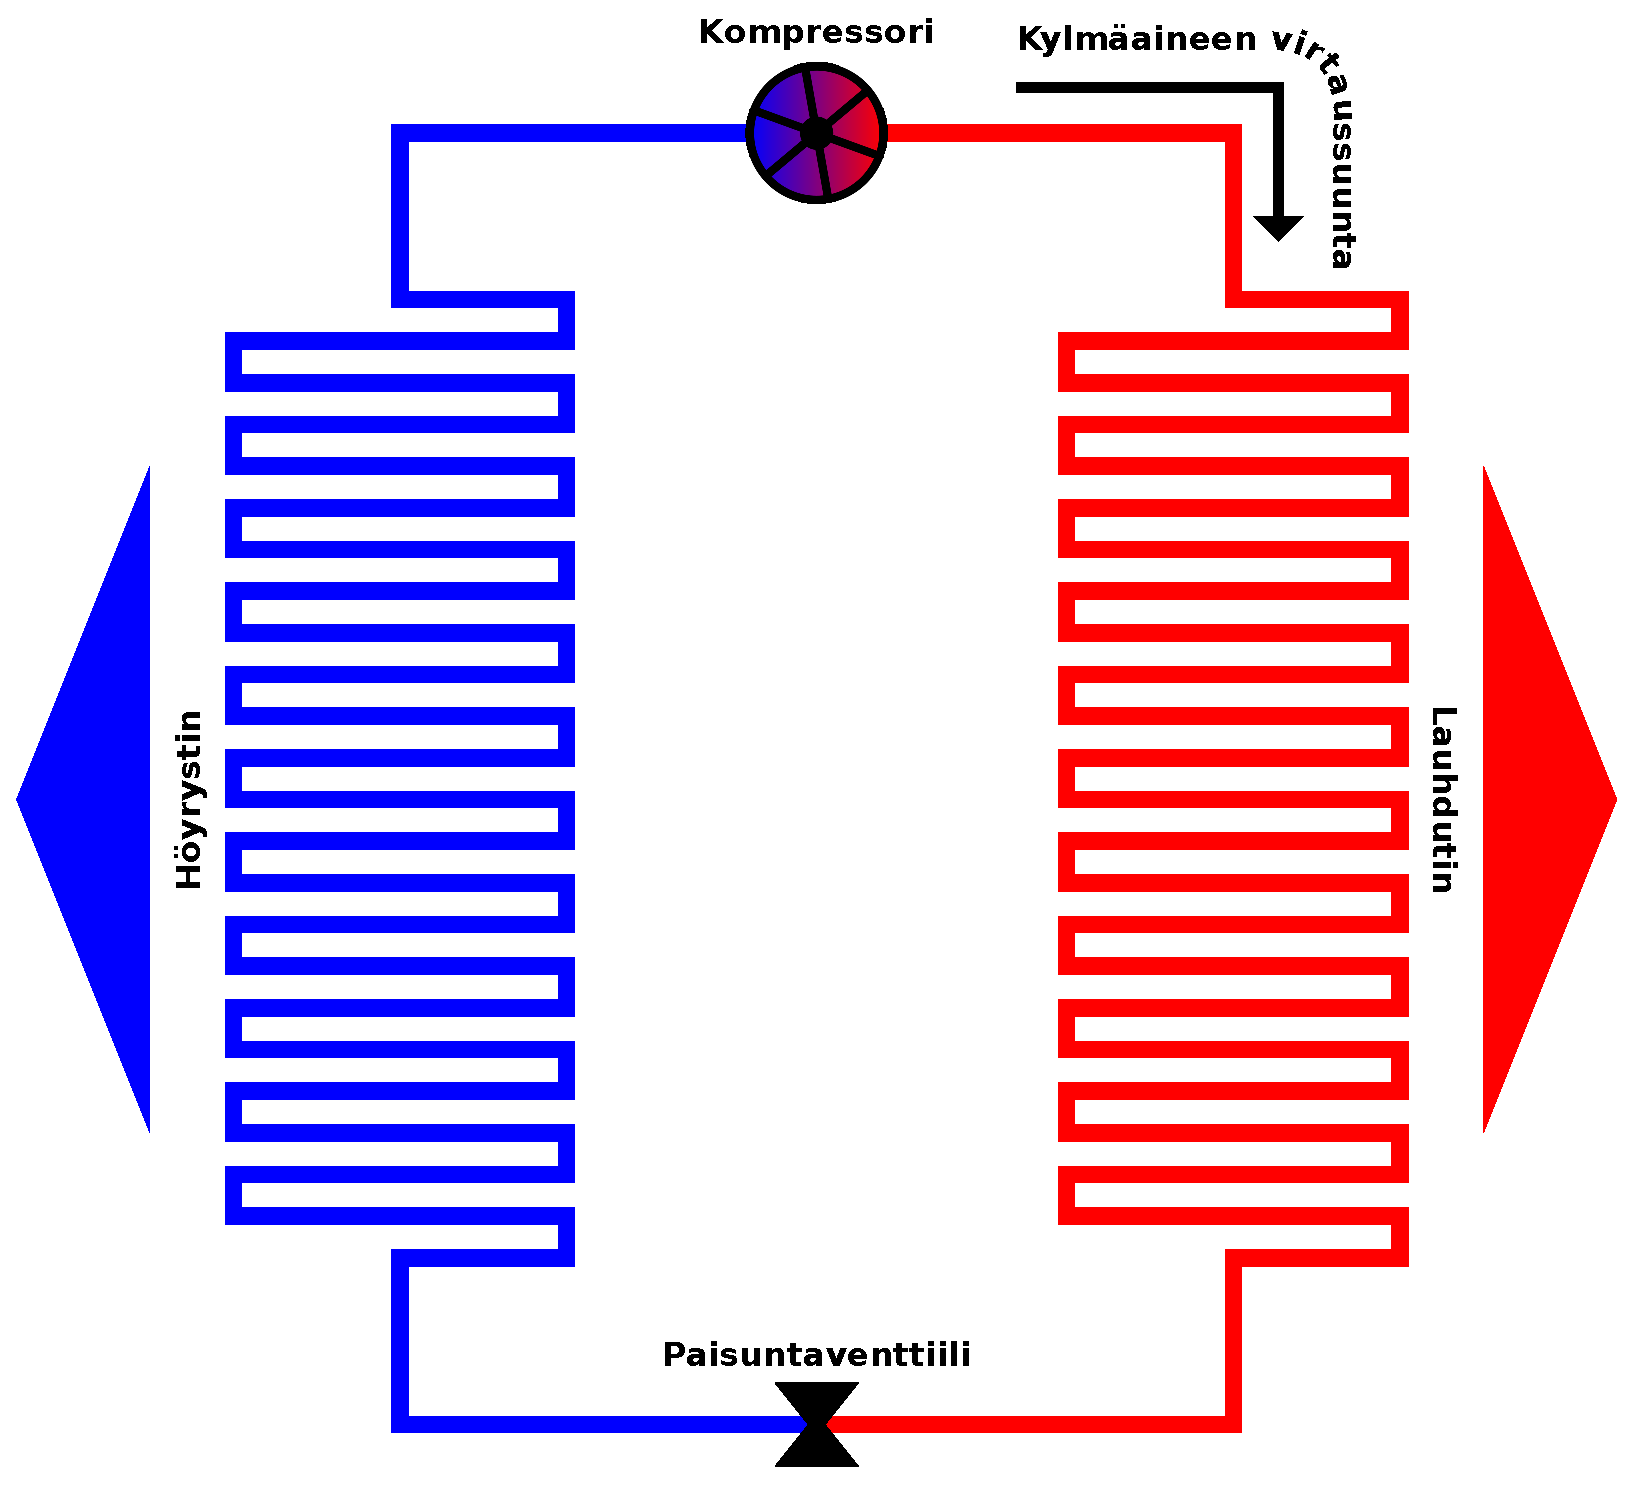
\includegraphics[width=0.5\textwidth]{figures/hp}
    \caption{Lämpöpumpun toimintaperiaate}
    \label{fig:hptp}
  \end{figure}

  Lämpöpumput käyttävät sähköenergiaa lämmön siirtämiseen viileämmästä lämpövarastosta lämpimämpään. Käytetystä sähköenergiasta valtaosa kuluu paineen tuottamiseen kompressorilla, mikä ylläpitää energiaa tuottavaa työkiertoa. Kompressorin lisäksi sähköä kuluu pienempiä määriä vaikkapa lämpöpumpun ohjaukseen, lämmitysjärjestelmän kiertovesipumpun käyttämiseen tai puhaltimen käyttämiseen. Mikäli lämpöpumpun teho on mitoitettu pienemmäksi kuin suurin vaadittu lämmitysteho\footnote{osatehomitoitus}, voidaan tehojen erotus tuottaa tarvittaessa lämpöpumpun yhteyteen asennettavilla sähkövastuksilla. Tällainen ratkaisu lisää huomattavasti järjestelmän sähkönkulutusta suurimman lämmitystarpeen aikana, jolloin sähköä käytetään muutenkin enemmän. Järjestelmän käyttäminen viilentämiseen taas lisää energian kulutusta, silloin kun sähkön käyttö on muuten todennäköisesti vähäisempää.

  Lämpöpumpuissa kompressorin pyörittämiseen käytetään sähkömoottoria. Vanhemmissa lämpöpumpuissa moottori on useimmiten verkkojännitteeseen kytketty oikosulkumoottori, joka voidaan tarvittaessa varustaa käynnistyksen ohjauksella eli pehmokäynnistimellä. Nykyaikaisemmassa ratkaisuissa oikosulkumoottoria käytetään taajuusmuuttajan avulla.

\section{Oikosulkumoottori}
  Yleisin tapa pyörittää lämpöpumpun kompressoria on käyttää suoraan verkkojännitteeseen kytkettyä oikosulkumoottoria. Kompressorin tehoa ei voida säädellä, vaan käydessään se tuottaa aina vakiotehon. Tällaisen lämpöpumpun tehoa säädetään kytkemällä kompressoria päälle ja pois. Kompressori kytkeytyy päälle, kun lämmitettävän kohteen, esimerkiksi lämminvesivaraajan tai sisäilman, lämpötila laskee tietyn rajan alapuolelle. Kun lämmitettävän kohteen lämpötila on noussut tarpeeksi, sammutetaan kompressori.

  Tärkeimmät kompressorin käyntijaksojen pituuteen vaikuttavat tekijät ovat lämmitettävän kohteen haluttu lämpötila ja lämpöenergian tarve, lämmönlähteen lämpötila ja kompressorin teho. Kotitalousköytössä kompressoreiden tehot ovat yleensä muutamia kilowatteja\footnote{etsi tarkempi tieto}.

  Mikäli oikosulkumoottorin käynnistysvirtaa ei mitenkään rajoiteta, on se tyypillisesti 6 -- 8 kertainen moottorin nimellisvirtaan nähden. Täten myös moottorin sähköverkosta käynnistyessään ottama teho on suuri.\parencite{pehmokaynnistinopas} Käynnistyksen jälkeen moottorin ottama virta ja teho laskevat kompressorin ottotehon määräämään arvoon.

  Oikosulkumoottorien suuret käynnistysvirrat näkyvät tehopiikkeinä myös sähköverkon puolella. Mikäli samassa muuntopiirissä on useampia lämpöpumppuja tai alhainen jännitejäykkyys, saattavat pumput aiheuttaa jännitetason vaihteluita. Alhaisen jännitejäykkyyden omaavissa verkoissa jo lämpöpumppujen normaalit käynnistykset saattavat aihetuttaa jännitetasonvaihteluita, jotka ilmenevät esimerkiksi välkyntänä\parencite{SFSEN50160}. Sähkökatkojen jälkeen kytkettäessä jännitettä takaisin, useat lämpöpumput saattavat käynnistyä samaan aikaan lämmittämään viilentyneitä lämmityskohteitaan. Tämä saattaa aiheuttaa lyhytaikaisen jännitteen aleneman. Mikäli jännitteenaleneman jälkeinen jäännösjännite on alle \SI{90}{\percent} järjestelmän nimellisjännitteestä, kutsutaan sitä jännitekuopaksi\parencite{SFSEN50160}.

  Oikosulkumoottoreiden käämityksistä johtuen ne ovat induktiivista kuormaa ja täten kuluttavat loistehoa. Mikäli moottoreiden kuluttamaa loistehoa ei kompensoida tuottamalla sitä paikallisesti, näyttäytyy lämpöpumppu sähköverkkoon induktiivisena kuormana. Induktiivisen kuorman kuluttama loisteho lisää häviöitä sähköverkossa ja loistehon kompensoinnin tarvertta verkkotasolla.\parencite{pakonen} \marginpar{onko kompensointia?}


\section{Oikosulkumoottori pehmokäynnistimellä}
  Lämpöpumpun käynnistyessään ottamaa virtapiikkiä voidaan pienentää tai se voidaan poistaa kokonaan pehmokäynnistimellä. Pehmokäynnistimen toiminta perustuu tyristoreihin, joilla säädellään moottorin kokemaa jännitettä. Alussa tyristorit johtavat vain hyvin pienen osan jännitteen jaksonajasta ja moottori alkaa tuottamaan momenttia. Vähitellen kasvatetaan tyristoreiden läpi päästettyä jännitteen osuutta, kunnes tyristorit ovat täysin johtavassa tilassa. Kun moottori on saavuttanut käyntinopeutensa, eivät tyristorit enää rajoita virtaa, ja ne voidaan esimerkiksi ohittaa kytkimellä tehohäviöiden pienentämiseksi.\parencite{pehmokaynnistinopas}

  Pehmokäynnistimen käyttö poistaa lämpöpumppujen käynnistysvirtapiikkien aiheuttaman ongelman. Pehmokäynnistimellä ei voida kuitenkaan järkevästi vaikuttaa moottorin käydessään ottamaan tehoon tai sen tuottamaan energiamäärään.

\section{Taajuusmuuttajakäytöt}
  Nykyaikainen ratkaisu lämpöpumpujen kompressorien käyttämiseen on taajuusmuuttaja. Taajuusmuuttaja koostuu tasasuuntaajasta ja ohjatusta vaihtosuuntaajasta, jolla saadaan tuotettua halutun suuruista ja taajuista vaihtojännitettä. Käynnistettäessä kompressoria aloitetaan moottorin syöttäminen matalataajuisella vaihtojännitteellä. Moottorin käyntinopeuden noustessa kohti haluttua arvoa, nostetaan samalla jännitteen taajuutta niin, että verkosta otettu teho pysyy suurin piirtein vakiona pyörimisnopeudesta riippumatta.

  Taajuusmuuttajan käytöllä saavutetaan useita hyötyjä. Käynnistysvirtapiikkien poistamisen lisäksi taajuusmuuttajalla voidaan myöskin säädellä kompressorin tuottamaa tehoa. Tehon säätäminen mahdollistaa pidemmät käyntijaksot ja tasaisemman tehonkulutuksen, mutta ei kuitenkaan vähennä lämpöpumpusta saatavaa maksimitehoa. Pienempien energiamäärien tuottaminen toteutetaan pienentämällä kompressorin käyntinopeutta, jolloin lämpöpumppua ei tarvitse käyttää useissa lyhyemmissä käyntijaksoissa.

  Verkon näkökulmasta taajuusmuuttaja näyttäytyy eri tavoilla riippuen siitä, miten siinä on totetutettu vaihtovirran tasasuuntaus. Perinteisissä ja halvemmissa taajuusmuuttajissa tasasuuntaus on toteutettu diodisillalla. Diodisilta aiheuttaa sisääntulevan virran säröytymistä ja sitä kautta myöskin jännitehäiriöitä verkkoon. Myöskään lämpöpumpun tehokertoimen säätäminen ei onnistu. Diodisiltaa parempi ratkaisu on verkkovaihtosuuntaaja, jonka ottama virta voidaan säätää lähes sinimuotoiseksi, jolloin virtasärön syntyminen voidaan ehkäistä. Verkkovaihtosuuntaajan tehokerrointa voidaan myöskin säätää, jolloin sitä voidaan käyttää loistehotasapainon ylläpitämiseen. Mikäli lämpöpumppua syöttävä taajuusmuuttaja on säädetty niin, että se näyttäytyy verkkoon lähes resistiivisenä kuormana se osaltaan vähentää verkon kuormitusta ja laskee jännitehäviöitä. Taajuusmuuttajan verkkoon aiheuttamat jännitehäiriöt riippuvat paljon taajuusmuuttajasta, sen laadusta ja koosta. \parencite{koskenjoki}

\section{Resistiivinen kuorma}
  Moottorikuormien lisäksi lämpöpumppujen yhteyteen asennetaan usein lämpövastuksia. Mikäli kyseessä on osatehomitoitettu lämpöpumppu, vastuksia käytetään suurimman energiatarpeen aikana, jolloin lämpöpumppu itsessään ei kykene tuottamaan kaikkea tarvittavaa energiaa. Lämpövastuksia käytetään myöskin höyrystimeen kertyneen jään ja huurteen poistoon.

  Lämpöpumpuissa kuluu sähköä myös muihin tarkoituksiin kuin suoraan energiantuotantoon. Automatiikan, ohjauksen ja sisä- ja ulkoyksiköiden puhaltimien kuluttama energia on kuitenkin vähäistä verrattuna muuhun energiankulutukseen
